
%(BEGIN_QUESTION)
% Copyright 2011, Tony R. Kuphaldt, released under the Creative Commons Attribution License (v 1.0)
% This means you may do almost anything with this work of mine, so long as you give me proper credit

Identify suitable input terminals, proper modes, and necessary connecting wires to allow this National Instruments E-series data acquisition unit (DAQ) to independently sense the voltages of the three series-connected solar cells shown:

$$\includegraphics[width=15.5cm]{i01616x01.eps}$$

The available modes for the input channels are RSE, NRSE, and DIFF:

% No blank lines allowed between lines of an \halign structure!
% I use comments (%) instead, so that TeX doesn't choke.

$$\vbox{\offinterlineskip
\halign{\strut
\vrule \quad\hfil # \ \hfil & 
\vrule \quad\hfil # \ \hfil & 
\vrule \quad\hfil # \ \hfil & 
\vrule \quad\hfil # \ \hfil \vrule \cr
\noalign{\hrule}
%
% First row
{\bf Channel} & {\bf Mode} & {\bf First terminal} & {\bf Second terminal} \cr
%
\noalign{\hrule}
%
% Another row
0 &  &  &  \cr
%
\noalign{\hrule}
%
% Another row
1 &  &  &  \cr
%
\noalign{\hrule}
%
% Another row
2 &  &  &  \cr
%
\noalign{\hrule}
} % End of \halign 
}$$ % End of \vbox

\vfil 

\underbar{file i01616}
\eject
%(END_QUESTION)





%(BEGIN_ANSWER)

This is a graded question -- no answers or hints given!

%(END_ANSWER)





%(BEGIN_NOTES)

Both Cell 1 and Cell 2 are {\it elevated} voltage sources, and thus cannot be read by the DAQ in any single-ended mode.  This means channels 1 and 2 must be configured as {\it differential}.  Cell 3 is a ground-referenced voltage source, and as such may be read in either single-ended or differential mode.

\vskip 10pt

This is one possible solution:

$$\includegraphics[width=15.5cm]{i01616x02.eps}$$

(The connection to ``AI Gnd'' is necessary to provide a bias current return path.)

% No blank lines allowed between lines of an \halign structure!
% I use comments (%) instead, so that TeX doesn't choke.

$$\vbox{\offinterlineskip
\halign{\strut
\vrule \quad\hfil # \ \hfil & 
\vrule \quad\hfil # \ \hfil & 
\vrule \quad\hfil # \ \hfil & 
\vrule \quad\hfil # \ \hfil \vrule \cr
\noalign{\hrule}
%
% First row
{\bf Channel} & {\bf Mode} & {\bf First terminal} & {\bf Second terminal} \cr
%
\noalign{\hrule}
%
% Another row
0 & DIFF & AI0 & AI8 \cr
%
\noalign{\hrule}
%
% Another row
1 & DIFF & AI1 & AI9 \cr
%
\noalign{\hrule}
%
% Another row
2 & DIFF & AI2 & AI10 \cr
%
\noalign{\hrule}
} % End of \halign 
}$$ % End of \vbox

\vfil \eject

Here is another possible solution:

$$\includegraphics[width=15.5cm]{i01616x03.eps}$$

(The connection to ``AI Gnd'' is necessary to provide a bias current return path.)

% No blank lines allowed between lines of an \halign structure!
% I use comments (%) instead, so that TeX doesn't choke.

$$\vbox{\offinterlineskip
\halign{\strut
\vrule \quad\hfil # \ \hfil & 
\vrule \quad\hfil # \ \hfil & 
\vrule \quad\hfil # \ \hfil & 
\vrule \quad\hfil # \ \hfil \vrule \cr
\noalign{\hrule}
%
% First row
{\bf Channel} & {\bf Mode} & {\bf First terminal} & {\bf Second terminal} \cr
%
\noalign{\hrule}
%
% Another row
0 & DIFF & AI0 & AI8 \cr
%
\noalign{\hrule}
%
% Another row
1 & DIFF & AI1 & AI9 \cr
%
\noalign{\hrule}
%
% Another row
2 & NRSE & AI2 & AI Sense \cr
%
\noalign{\hrule}
} % End of \halign 
}$$ % End of \vbox


%INDEX% Pictorial circuit review (analog signal wiring to data acquisition unit)

%(END_NOTES)

